
\begin{correction}   \;
\begin{enumerate}
%--------------------------------------------------
\item \textbf{R\'esolution de $\mathbf{\cos{(3x-2)}=\cos{(2x-1)}}$:}\\
\noindent On sait que $\cos{(X)}=\cos{(Y)}\Leftrightarrow \left\lbrace\begin{array}{llll}  \exists k\in\Z,& X&=& Y+2k\pi\vsec\\
\hbox{ou}\vsec\\
 \exists k\in\Z,& X&=& -Y+2k\pi.    \end{array}\right.$ On peut appliquer cela ici et on obtient:
$$\cos{(3x-2)}=\cos{(2x-1)}\Leftrightarrow \left\lbrace\begin{array}{llll}  \exists k\in\Z,& 3x-2&=& 2x-1+2k\pi\vsec\\ \hbox{ou}\vsec\\  \exists k\in\Z,& 3x-2&=& -2x+1+2k\pi    \end{array}\right. \Leftrightarrow \left\lbrace\begin{array}{llll}  \exists k\in\Z,& x&=& 1+2k\pi\vsec\\ \hbox{ou}\vsec\\\exists k\in\Z,& x&=& \ddp\frac{3}{5}+\ddp\frac{2k\pi}{5}.    \end{array}\right.$$
\begin{minipage}[c]{0.45\textwidth}
On obtient ainsi:
$$\fbox{$\mathcal{S}_{\R}=\left\lbrace 1+2k\pi,\ k\in\Z\right\rbrace\cup\left\lbrace \ddp\frac{3}{5}+\ddp\frac{2k\pi}{5},\ k\in\Z\right\rbrace$}.$$
Et on a :
$$\fbox{$\mathcal{S}_{[0,2\pi[}=\left\{ 1, \ddp\frac{3}{5}, \ddp\frac{3}{5}+\ddp\frac{2\pi}{5}, \ddp\frac{3}{5}+\ddp\frac{4\pi}{5}, \ddp\frac{3}{5}+\ddp\frac{6\pi}{5}, \ddp\frac{3}{5}+\ddp\frac{8\pi}{5} \right\}$}.$$
\end{minipage}
\quad \begin{minipage}[c]{0.45\textwidth}
\begin{center}
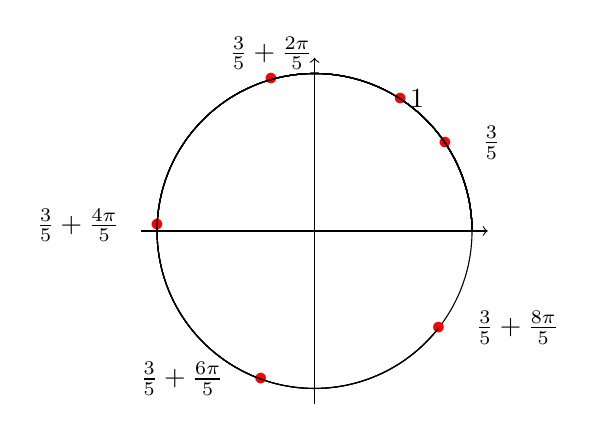
\begin{tikzpicture}[scale=2]
%Axes
\draw [->] (-1.1,0) -- (1.1,0);
\draw [->] (0,-1.1) -- (0,1.1);
%Cercle
\draw (0,0) circle (1);
%Points
\draw (1,0) arc (0:57:1) node [red] {$\bullet$};
\draw (1,0) arc (0:57:1) node[right] {$\ddp 1$} ;
\draw (1,0) arc (0:34:1) node [red] {$\bullet$};
\draw (1,0) arc (0:34:1) node[right] {$\quad \ddp \frac{3}{5}$} ;
\draw (1,0) arc (0:106:1) node [red] {$\bullet$};
\draw (1,0) arc (0:106:1) node[above] {$\ddp \frac{3}{5} + \frac{2\pi}{5}$} ;
\draw (1,0) arc (0:178:1) node [red] {$\bullet$};
\draw (1,0) arc (0:178:1) node[left] {$\ddp \frac{3}{5} + \frac{4\pi}{5}\quad$} ;
\draw (1,0) arc (0:250:1) node [red] {$\bullet$};
\draw (1,0) arc (0:250:1) node[left] {$\ddp \frac{3}{5} + \frac{6\pi}{5}\quad$} ;
\draw (1,0) arc (0:322:1) node [red] {$\bullet$};
\draw (1,0) arc (0:322:1) node[right] {$\quad \ddp \frac{3}{5} + \frac{8\pi}{5}$} ;
\end{tikzpicture}
\end{center}
\end{minipage}
%--------------------------------------------------
\item \textbf{R\'esolution de $\mathbf{\sin{\left(3x-\ddp\frac{\pi}{3}\right)}=\sin{\left(2x+\ddp\frac{\pi}{6}\right)}}$:}\\
\noindent De m\^{e}me, on sait que $\sin{(X)}=\sin{(Y)}\Leftrightarrow \left\lbrace\begin{array}{llll}  \exists k\in\Z,& X&=& Y+2k\pi\vsec\\ \hbox{ou}\vsec\\ \exists k\in\Z,& X&=& \pi-Y+2k\pi.    \end{array}\right.$ On peut appliquer cela ici et on obtient:
$$\sin{\left(3x-\ddp\frac{\pi}{3}\right)}=\sin{\left(2x+\ddp\frac{\pi}{6}\right)} \Leftrightarrow \left\lbrace\begin{array}{llll}  \exists k\in\Z,& 3x-\ddp\frac{\pi}{3}&=& 2x+\ddp\frac{\pi}{6}+2k\pi\vsec\\ \hbox{ou}\vsec\\ \exists k\in\Z,& 3x-\ddp\frac{\pi}{3}&=&\pi-2x-\ddp\frac{\pi}{6}+2k\pi    \end{array}\right. \Leftrightarrow \left\lbrace\begin{array}{llll}  \exists k\in\Z,& x&=& \ddp\frac{\pi}{2}+2k\pi\vsec\\ \hbox{ou}\vsec\\\exists k\in\Z,& x&=& \ddp\frac{7\pi}{30}+\ddp\frac{2k\pi}{5}.    \end{array}\right.$$
\begin{minipage}[c]{0.45\textwidth}
On obtient ainsi:
$$\fbox{$\mathcal{S}_{\R}=\left\lbrace \ddp\frac{\pi}{2}+2k\pi,\ k\in\Z\right\rbrace\cup\left\lbrace \ddp\frac{7\pi}{30}+\ddp\frac{2k\pi}{5},\ k\in\Z\right\rbrace$.}$$
Et on a :
$$\fbox{$\mathcal{S}_{[0,2\pi[}=\left\{ \ddp \frac{\pi}{2}, \frac{7\pi}{30}, \frac{19\pi}{30}, \frac{31\pi}{30}, \frac{43\pi}{30}, \frac{55\pi}{30}\right\}$}.$$
\end{minipage}
\quad \begin{minipage}[c]{0.45\textwidth}
\begin{center}
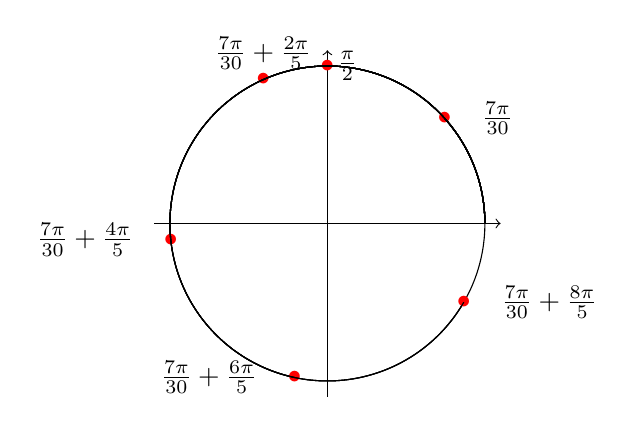
\begin{tikzpicture}[scale=2]
%Axes
\draw [->] (-1.1,0) -- (1.1,0);
\draw [->] (0,-1.1) -- (0,1.1);
%Cercle
\draw (0,0) circle (1);
%Points
\draw (1,0) arc (0:90:1) node [red] {$\bullet$};
\draw (1,0) arc (0:90:1) node[right] {$\ddp \frac{\pi}{2}$} ;
\draw (1,0) arc (0:42:1) node [red] {$\bullet$};
\draw (1,0) arc (0:42:1) node[right] {$\quad \ddp \frac{7\pi}{30}$} ;
\draw (1,0) arc (0:114:1) node [red] {$\bullet$};
\draw (1,0) arc (0:114:1) node[above] {$\ddp \frac{7\pi}{30} + \frac{2\pi}{5}$} ;
\draw (1,0) arc (0:186:1) node [red] {$\bullet$};
\draw (1,0) arc (0:186:1) node[left] {$\ddp \frac{7\pi}{30} + \frac{4\pi}{5}\quad$} ;
\draw (1,0) arc (0:258:1) node [red] {$\bullet$};
\draw (1,0) arc (0:258:1) node[left] {$\ddp \frac{7\pi}{30} + \frac{6\pi}{5}\quad$} ;
\draw (1,0) arc (0:330:1) node [red] {$\bullet$};
\draw (1,0) arc (0:330:1) node[right] {$\quad \ddp \frac{7\pi}{30} + \frac{8\pi}{5}$} ;
\end{tikzpicture}
\end{center}
\end{minipage}
%--------------------------------------------------
\item \textbf{R\'esolution de $\mathbf{\tan{(x+1)}+\tan{(3x+1)}=0}$:}
\begin{itemize}
\item[$\bullet$] On commence par rechercher le domaine de d\'efinition de cette \'equation. On doit donc avoir pour tout $k\in\Z$: $x+1\not= \ddp\frac{\pi}{2}+k\pi$ et $3x+1\not= \ddp\frac{\pi}{2}+k\pi$. On obtient donc que $\mathcal{D}=\R \setminus\left\lbrace  \ddp\frac{\pi}{2}-1+k\pi;\ddp\frac{\pi}{6}-\ddp\frac{1}{3}+\ddp\frac{k\pi}{3},\ k\in\Z  \right\rbrace$. 
\item[$\bullet$] De m\^{e}me que dans les deux exemples pr\'ec\'edents, on sait que $\tan{(X)}=\tan{(Y)}\Leftrightarrow \exists k\in\Z,\ X=Y+k\pi$. On peut appliquer cela ici et on obtient en utilisant tout d'abord l'imparit\'e de la tangente:
$$\begin{array}{lll} \tan{(x+1)}+\tan{(3x+1)}=0&\Leftrightarrow &\tan{(x+1)}=-\tan{(3x+1)} \Leftrightarrow  \tan{(x+1)}=\tan{(-3x-1)} \vsec\\
&\Leftrightarrow &\exists k\in\Z,\ x+1=-3x-1+k\pi\Leftrightarrow \exists k\in\Z,\ x=-\ddp\demi+\ddp\frac{k\pi}{4}.\end{array}$$
\end{itemize}
\begin{minipage}[c]{0.45\textwidth}
Comme pour tout $k\in\Z:$ $-\ddp\demi+\ddp\frac{k\pi}{4}\in\mathcal{D}$, on obtient:
$$\fbox{$\mathcal{S}_{\R}=\left\lbrace -\ddp\demi+\ddp\frac{k\pi}{4},\ k\in\Z\right\rbrace$}.$$
Et on a :
$$\fbox{$\mathcal{S}_{[0,2\pi[}=\left\{ - \ddp\frac{1}{2}, - \ddp\frac{1}{2}+\ddp\frac{\pi}{4},  - \ddp\frac{1}{2}+\ddp\frac{\pi}{2},  - \ddp\frac{1}{2}+\ddp\frac{3\pi}{4} \right\}$}.$$
\end{minipage}
\quad \begin{minipage}[c]{0.45\textwidth}
\begin{center}
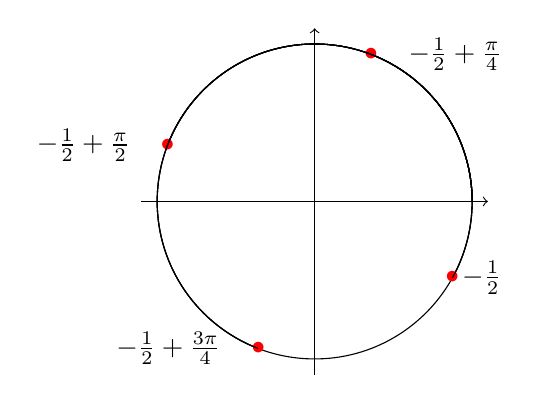
\begin{tikzpicture}[scale=2]
%Axes
\draw [->] (-1.1,0) -- (1.1,0);
\draw [->] (0,-1.1) -- (0,1.1);
%Cercle
\draw (0,0) circle (1);
%Points
\draw (1,0) arc (0:-29:1) node [red] {$\bullet$};
\draw (1,0) arc (0:-29:1) node[right] {$\ddp - \frac{1}{2}$} ;
\draw (1,0) arc (0:69:1) node [red] {$\bullet$};
\draw (1,0) arc (0:69:1) node[right] {$\quad \ddp - \ddp\frac{1}{2}+\ddp\frac{\pi}{4}$} ;
\draw (1,0) arc (0:159:1) node [red] {$\bullet$};
\draw (1,0) arc (0:159:1) node[left] {$\ddp - \ddp\frac{1}{2}+\ddp\frac{\pi}{2}\quad$} ;
\draw (1,0) arc (0:249:1) node [red] {$\bullet$};
\draw (1,0) arc (0:249:1) node[left] {$\ddp - \ddp\frac{1}{2}+\ddp\frac{3\pi}{4} \quad$} ;
\end{tikzpicture}
\end{center}
\end{minipage}
%--------------------------------------------------
\item \textbf{R\'esolution de $\mathbf{\sin^2{x}=\ddp\demi}$:}\\
\noindent  En posant $X=\sin{(x)}$, on doit r\'esoudre $X^2=\ddp\demi$, \`{a} savoir: $X=\ddp\frac{1}{\sqrt{2}}$ ou $X=-\ddp\frac{1}{\sqrt{2}}$. On doit donc r\'esoudre $\sin{(x)}=\ddp\frac{1}{\sqrt{2}}$ ou $\sin{(x)}=-\ddp\frac{1}{\sqrt{2}}$. On obtient ainsi
$$\fbox{$\mathcal{S}_{\R}=\left\lbrace  -\ddp\frac{3\pi}{4}+2k\pi,\ k\in\Z \right\rbrace \cup\left\lbrace  -\ddp\frac{\pi}{4}+2k\pi,\ k\in\Z \right\rbrace \cup\left\lbrace  \ddp\frac{\pi}{4}+2k\pi,\ k\in\Z \right\rbrace \cup\left\lbrace  \ddp\frac{3\pi}{4}+2k\pi,\ k\in\Z \right\rbrace$}$$
\begin{minipage}[c]{0.45\textwidth}
Et on a :
$$\fbox{$ \mathcal{S}_{\lbrack 0,2\pi\lbrack}=\left\lbrace \ddp\frac{\pi}{4},\ddp\frac{3\pi}{4},\ddp\frac{5\pi}{4},\ddp\frac{7\pi}{4}  \right\rbrace$}.$$
\end{minipage}
\quad \begin{minipage}[c]{0.45\textwidth}
\begin{center}
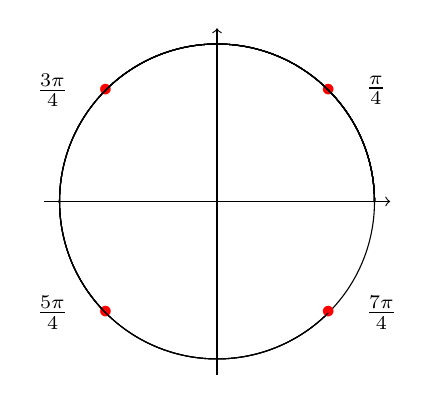
\begin{tikzpicture}[scale=2]
%Axes
\draw [->] (-1.1,0) -- (1.1,0);
\draw [->] (0,-1.1) -- (0,1.1);
%Cercle
\draw (0,0) circle (1);
%Points
\draw (1,0) arc (0:45:1) node [red] {$\bullet$};
\draw (1,0) arc (0:45:1) node[right] {$\quad\ddp \frac{\pi}{4}$} ;
\draw (1,0) arc (0:135:1) node [red] {$\bullet$};
\draw (1,0) arc (0:135:1) node[left] {$\ddp \ddp\frac{3\pi}{4}\quad$} ;
\draw (1,0) arc (0:225:1) node [red] {$\bullet$};
\draw (1,0) arc (0:225:1) node[left] {$\ddp \ddp\frac{5\pi}{4}\quad$} ;
\draw (1,0) arc (0:315:1) node [red] {$\bullet$};
\draw (1,0) arc (0:315:1) node[right] {$\quad \ddp \ddp\frac{7\pi}{4}$} ;
\end{tikzpicture}
\end{center}
\end{minipage}
%--------------------------------------------------
\item \textbf{R\'esolution de $\mathbf{\sin{(2x)}=\cos{\left(\ddp\frac{x}{2}\right)}}$:}\\
\noindent Une fa\c{c}on de faire ici est de transformer le cosinus en sinus. On obtient ainsi
$$\begin{array}{lll}\sin{(2x)}=\cos{\left(\ddp\frac{x}{2}\right)} &\Leftrightarrow &\sin{(2x)}=\sin{\left(\ddp\frac{\pi}{2}+\ddp\frac{x}{2}\right)} \Leftrightarrow \left\lbrace\begin{array}{llll}  \exists k\in\Z,& 2x&=& \ddp\frac{\pi}{2}+\ddp\frac{x}{2}+2k\pi\vsec\\ \hbox{ou}\vsec\\ \exists k\in\Z,& 2x&=&\pi-\ddp\frac{\pi}{2}-\ddp\frac{x}{2}+2k\pi    \end{array}\right. \vsec\\
&\Leftrightarrow & \left\lbrace\begin{array}{llll}  \exists k\in\Z,& x&=& \ddp\frac{\pi}{3}+\ddp\frac{4k\pi}{3}\vsec\\ \hbox{ou}\vsec\\ \exists k\in\Z,& x&=& \ddp\frac{\pi}{5}+\ddp\frac{4k\pi}{5}.    \end{array}\right.\end{array}$$
 \begin{minipage}[c]{0.45\textwidth}
On obtient ainsi:
$$\fbox{$\mathcal{S}_{\R}=\left\lbrace  \ddp\frac{\pi}{3}+\ddp\frac{4k\pi}{3} ,\ k\in\Z\right\rbrace\cup\left\lbrace  \ddp\frac{\pi}{5}+\ddp\frac{4k\pi}{5},\ k\in\Z\right\rbrace$}.$$
Et on a :
$$\fbox{$\mathcal{S}_{\lbrack 0,2\pi\lbrack}=\left\lbrace 
\ddp\frac{\pi}{5},\ddp\frac{\pi}{3},\ddp\frac{3\pi}{5},\ddp\frac{7\pi}{5},\pi,\ddp\frac{5\pi}{3},\ddp\frac{9\pi}{5}\right\rbrace$}.$$
\end{minipage}
\quad \begin{minipage}[c]{0.45\textwidth}
\begin{center}
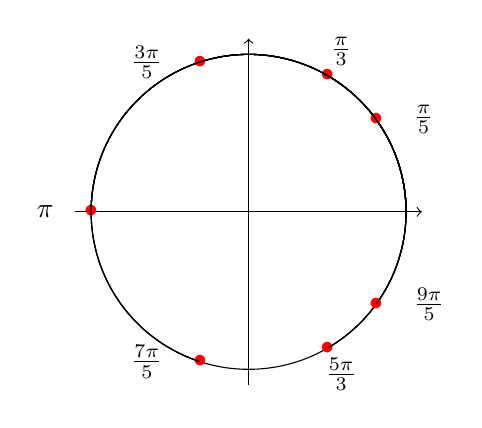
\begin{tikzpicture}[scale=2]
%Axes
\draw [->] (-1.1,0) -- (1.1,0);
\draw [->] (0,-1.1) -- (0,1.1);
%Cercle
\draw (0,0) circle (1);
%Points
\draw (1,0) arc (0:60:1) node [red] {$\bullet$};
\draw (1,0) arc (0:60:1) node[above] {$\quad\ddp \frac{\pi}{3}$} ;
\draw (1,0) arc (0:180:1) node [red] {$\bullet$};
\draw (1,0) arc (0:180:1) node[left] {$\ddp \pi \quad$} ;
\draw (1,0) arc (0:-60:1) node [red] {$\bullet$};
\draw (1,0) arc (0:-60:1) node[below] {$\quad \ddp \ddp\frac{5\pi}{3}$} ;
\draw (1,0) arc (0:36:1) node [red] {$\bullet$};
\draw (1,0) arc (0:36:1) node[right] {$\quad \ddp \ddp\frac{\pi}{5}$} ;
\draw (1,0) arc (0:108:1) node [red] {$\bullet$};
\draw (1,0) arc (0:108:1) node[left] {$ \ddp \ddp\frac{3\pi}{5} \quad$} ;
\draw (1,0) arc (0:252:1) node [red] {$\bullet$};
\draw (1,0) arc (0:252:1) node[left] {$ \ddp \ddp\frac{7\pi}{5}\quad$} ;
\draw (1,0) arc (0:-36:1) node [red] {$\bullet$};
\draw (1,0) arc (0:-36:1) node[right] {$\quad \ddp \ddp\frac{9\pi}{5}$} ;
\end{tikzpicture}
\end{center}
\end{minipage}
%--------------------------------------------------
\item \textbf{R\'esolution de $\mathbf{ 2\cos^2{(3x)}+3\cos{(3x)}+1=0    }$:}\\
\noindent On pose le changement de variable $X=\cos{(3x)}$ et on doit donc r\'esoudre $2X^2+3X+1=0$. Le discriminant vaut $\Delta=1$ et les deux solutions distinctes sont donc $X_1=-1$ et $X_2=-\ddp\demi$. Ainsi on doit donc r\'esoudre $\cos{(3x)}=-1$ et $\cos{(3x)}=-\ddp\demi$. La r\'esolution de ces deux \'equations fondamentales donne 
$$ \fbox{$\mathcal{S}_{\R}=\left\lbrace  \ddp\frac{\pi}{3}+\ddp\frac{2k\pi}{3} ,\ k\in\Z\right\rbrace\cup\left\lbrace  \ddp\frac{2\pi}{9}+\ddp\frac{2k\pi}{3},\ k\in\Z\right\rbrace\cup\left\lbrace  -\ddp\frac{2\pi}{9}+\ddp\frac{2k\pi}{3},\ k\in\Z\right\rbrace$}.$$
\begin{minipage}[c]{0.45\textwidth}
Et on a :
$$ \fbox{$\mathcal{S}_{\lbrack 0,2\pi\lbrack}=\left\lbrace \ddp\frac{2\pi}{9} , \ddp\frac{\pi}{3},\ddp\frac{4\pi}{9} ,\ddp\frac{8\pi}{9},\pi,\ddp\frac{10\pi}{9},\ddp\frac{14\pi}{9},\ddp\frac{5\pi}{3},\ddp\frac{16\pi}{9} \right\rbrace .$}$$
\end{minipage}
\quad \begin{minipage}[c]{0.45\textwidth}
\begin{center}
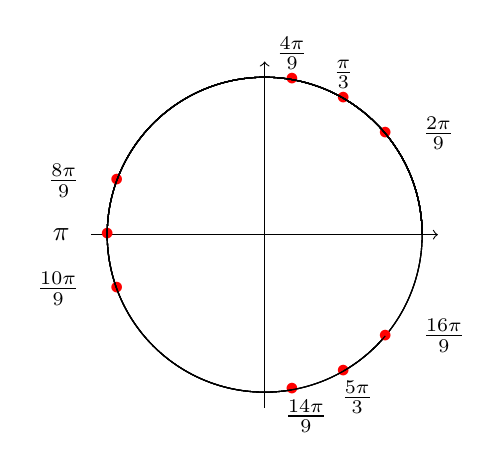
\begin{tikzpicture}[scale=2]
%Axes
\draw [->] (-1.1,0) -- (1.1,0);
\draw [->] (0,-1.1) -- (0,1.1);
%Cercle
\draw (0,0) circle (1);
%Points
\draw (1,0) arc (0:60:1) node [red] {$\bullet$};
\draw (1,0) arc (0:60:1) node[above] {$\ddp \frac{\pi}{3}$} ;
\draw (1,0) arc (0:180:1) node [red] {$\bullet$};
\draw (1,0) arc (0:180:1) node[left] {$\ddp \pi \quad$} ;
\draw (1,0) arc (0:-60:1) node [red] {$\bullet$};
\draw (1,0) arc (0:-60:1) node[below] {$\quad \ddp \ddp\frac{5\pi}{3}$} ;
\draw (1,0) arc (0:40:1) node [red] {$\bullet$};
\draw (1,0) arc (0:40:1) node[right] {$\quad \ddp \ddp\frac{2\pi}{9}$} ;
\draw (1,0) arc (0:80:1) node [red] {$\bullet$};
\draw (1,0) arc (0:80:1) node[above] {$ \ddp \ddp\frac{4\pi}{9}$} ;
\draw (1,0) arc (0:160:1) node [red] {$\bullet$};
\draw (1,0) arc (0:160:1) node[left] {$ \ddp \ddp\frac{8\pi}{9} \quad$} ;
\draw (1,0) arc (0:200:1) node [red] {$\bullet$};
\draw (1,0) arc (0:200:1) node[left] {$ \ddp \ddp\frac{10\pi}{9} \quad$} ;
\draw (1,0) arc (0:280:1) node [red] {$\bullet$};
\draw (1,0) arc (0:280:1) node[below] {$\quad \ddp \ddp\frac{14\pi}{9} $} ;
\draw (1,0) arc (0:320:1) node [red] {$\bullet$};
\draw (1,0) arc (0:320:1) node[right] {$\quad \ddp \ddp\frac{16\pi}{9} $} ;
\end{tikzpicture}
\end{center}
\end{minipage}
%--------------------------------------------------
%\item \textbf{R\'esolution de $\mathbf{\sin{x}+\ddp\frac{1}{\sqrt{3}}\cos{x}=-1}$:}\\
%\noindent M\^{e}me m\'ethode que dans l'exercice 3. On ne donne que la solution:
%\begin{equation*}
%\fbox{
%$\mathcal{S}_{\R}=\left\lbrace \ddp\frac{7\pi}{6}+2k\pi,\ k\in\Z  \right\rbrace\cup \left\lbrace -\ddp\frac{\pi}{2}+2k\pi,\ k\in\Z  \right\rbrace\ \hbox{et}\  \mathcal{S}_{\lbrack 0,2\pi\lbrack}=\left\lbrace \ddp\frac{7\pi}{6} , \ddp\frac{3\pi}{2}  \right\rbrace.$}
%\end{equation*}
%--------------------------------------------------
\item \textbf{R\'esolution de $\mathbf{2\sin^2{x}=\sqrt{3}\sin{(2x)} }$:}\\
\noindent En utilisant la formule de duplication du sinus, on obtient la factorisation suivante
$$\begin{array}{lll}
2\sin^2{x}=\sqrt{3}\sin{(2x)}& \Leftrightarrow& \sin{x}\left(\sin{x}-\sqrt{3}\cos{x} \right)=0\vsec\\
&\Leftrightarrow & \sin{x}=0\ \hbox{ou}\ \sin{x}-\sqrt{3}\cos{x}=0\vsec\\
&\Leftrightarrow & \exists k\in\Z,\  x=k\pi \ \hbox{ou}\ \sin{x}-\sqrt{3}\cos{x}=0.
\end{array}$$
La deuxi\`eme \'equation est de type $a\cos{x}+b\sin{x}$. On obtient :
$$\begin{array}{lll}
\sin{x}-\sqrt{3}\cos{x}&=&2\left( -\ddp\frac{\sqrt{3}}{2}\cos{x}+\frac{1}{2}\sin{x}   \right)
= 2\cos{\left(x-\ddp\frac{5\pi}{6}\right)}.
\end{array}$$
Ainsi,
$$\begin{array}{lll}
2\sin^2{x}=\sqrt{3}\sin{(2x)}& \Leftrightarrow& \exists k\in\Z,\  x=k\pi \ \hbox{ou}\ \cos{\left(x-\ddp\frac{5\pi}{6}\right)}=0
\Leftrightarrow \left\lbrace \begin{array}{llll}
\exists k\in\Z,&  x&=&k\pi\\
\hbox{ou}\\
\exists k\in\Z,&  x&=&\ddp\frac{4\pi}{3}+2k\pi\\
\hbox{ou}\\
\exists k\in\Z,& x&=&\ddp\frac{\pi}{3}+2k\pi\\
\end{array}\right.
\end{array}$$
On a donc :
$$\fbox{$\mathcal{S}_{\R}=\left\lbrace k\pi,\ k\in\Z  \right\rbrace\cup \left\lbrace \ddp\frac{4\pi}{3}+2k\pi,\ k\in\Z  \right\rbrace\cup \left\lbrace \ddp\frac{\pi}{3}+2k\pi,\ k\in\Z  \right\rbrace$}.$$
\begin{minipage}[c]{0.45\textwidth}
Et de plus :
$$\fbox{$\mathcal{S}_{\lbrack 0,2\pi\lbrack}=\left\lbrace 0,\ddp\frac{\pi}{3},\pi,\ddp\frac{4\pi}{3} \right\rbrace$}.$$
\end{minipage}
\quad \begin{minipage}[c]{0.45\textwidth}
\begin{center}
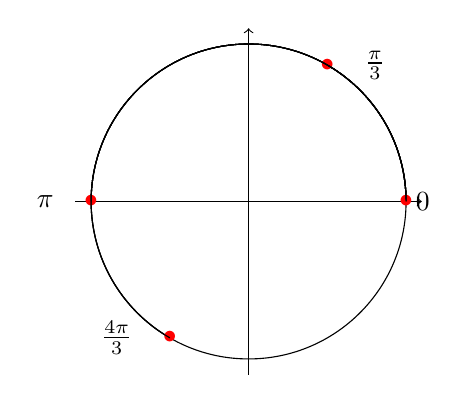
\begin{tikzpicture}[scale=2]
%Axes
\draw [->] (-1.1,0) -- (1.1,0);
\draw [->] (0,-1.1) -- (0,1.1);
%Cercle
\draw (0,0) circle (1);
%Points
\draw (1,0) arc (0:60:1) node [red] {$\bullet$};
\draw (1,0) arc (0:60:1) node[right] {$\quad \ddp \frac{\pi}{3}$} ;
\draw (1,0) arc (0:180:1) node [red] {$\bullet$};
\draw (1,0) arc (0:180:1) node[left] {$\ddp \pi \quad$} ;
\draw (1,0) arc (0:0:1) node [red] {$\bullet$};
\draw (1,0) arc (0:0:1) node[right] {$\ddp 0$} ;
\draw (1,0) arc (0:240:1) node [red] {$\bullet$};
\draw (1,0) arc (0:240:1) node[left] {$\ddp \ddp\frac{4\pi}{3}\quad$} ;
\end{tikzpicture}
\end{center}
\end{minipage}
%-----------------------------------
\item \textbf{R\'esolution de $\mathbf{ \sin{\left(2x-\ddp\frac{\pi}{4}\right)}=-\cos{\left(x+\ddp\frac{\pi}{6}\right)} }$:}\\
\noindent
On transforme le cosinus en sinus afin de se ramener \`a une \'equation fondamentale.
On a en utilisant l'imparit\'e du sinus:
$$
\sin{\left(2x-\ddp\frac{\pi}{4}\right)}=-\sin{\left(\ddp\frac{\pi}{2}-x-\frac{\pi}{6}\right)}
=\sin{\left(-\ddp\frac{\pi}{2}+x+\frac{\pi}{6}\right)}
=\sin{\left(x-\ddp\frac{\pi}{3}\right)}.$$
Ainsi,
$$
\sin{\left(2x-\ddp\frac{\pi}{4}\right)}=-\cos{\left(x+\ddp\frac{\pi}{6}\right)} \Leftrightarrow  \left\lbrace \begin{array}{l}
\exists k\in\Z,\ 2x-\ddp\frac{\pi}{4}=x-\ddp\frac{\pi}{3}+2k\pi\vsec\\
\hbox{ou}\vsec\\
\exists k\in\Z,\ 2x-\ddp\frac{\pi}{4}=\pi-x+\ddp\frac{\pi}{3}+2k\pi,
\end{array}\right.
\Leftrightarrow \left\lbrace\begin{array}{llll}
\exists k\in\Z, &x&=&-\ddp\frac{\pi}{12}+2k\pi\\
\hbox{ou}\\
\exists k\in\Z,& x&=&-\ddp\frac{5\pi}{36}+\frac{2k\pi}{3}.\\
\end{array}\right.$$
\begin{minipage}[c]{0.45\textwidth}
On obtient :
$$\fbox{$\mathcal{S}_{\R}=\left\lbrace -\ddp\frac{\pi}{12}+2k\pi,\ k\in\Z  \right\rbrace\cup \left\lbrace \ddp\frac{19\pi}{36}+\frac{2k\pi}{3},\ k\in\Z  \right\rbrace$}.$$ 
Et on a :
$$\fbox{$\mathcal{S}_{\lbrack 0,2\pi\lbrack}=\left\lbrace \ddp\frac{19\pi}{36}, \ddp\frac{43\pi}{36} ,\ddp\frac{67\pi}{36},\ddp\frac{23\pi}{12} \right\rbrace$}.$$
\end{minipage}
\quad \begin{minipage}[c]{0.45\textwidth}
\begin{center}
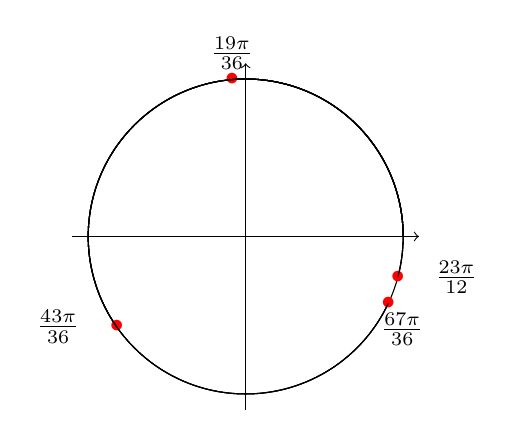
\begin{tikzpicture}[scale=2]
%Axes
\draw [->] (-1.1,0) -- (1.1,0);
\draw [->] (0,-1.1) -- (0,1.1);
%Cercle
\draw (0,0) circle (1);
%Points
\draw (1,0) arc (0:95:1) node [red] {$\bullet$};
\draw (1,0) arc (0:95:1) node[above] {$\ddp \frac{19\pi}{36}$} ;
\draw (1,0) arc (0:215:1) node [red] {$\bullet$};
\draw (1,0) arc (0:215:1) node[left] {$\ddp \frac{43\pi}{36} \quad$} ;
\draw (1,0) arc (0:335:1) node [red] {$\bullet$};
\draw (1,0) arc (0:335:1) node[below] {$\quad \ddp \frac{67\pi}{36}$} ;
\draw (1,0) arc (0:-15:1) node [red] {$\bullet$};
\draw (1,0) arc (0:-15:1) node[right] {$\quad\ddp \ddp\frac{23\pi}{12}$} ;
\end{tikzpicture}
\end{center}
\end{minipage}
%--------------------------------------------------
\item \textbf{R\'esolution de $\mathbf{\sqrt{3}\cos^2{x}+2\cos{x}\sin{x}-\sqrt{3}\sin^2{x}=\sqrt{2}}$:}\\
\noindent On commence par utiliser le formulaire de trigonom\'etrie afin de transformer l'expression:
$$\sqrt{3}\cos^2{x}+2\cos{x}\sin{x}-\sqrt{3}\sin^2{x}=\sqrt{3}\left(\cos^2{x}-\sin^2{x}  \right)+\sin{(2x)}=\sqrt{3}\cos{(2x)}+\sin{(2x)}.$$
On pose $X=2x$, et on factorise $\sqrt{3}\cos{(2x)}+\sin{(2x)}$. \\
\begin{minipage}[c]{0.45\textwidth}
On obtient :
$$\fbox{$\mathcal{S}_{\R}= \left\lbrace \ddp\frac{5\pi}{24}+k\pi,\ k\in\Z  \right\rbrace\cup \left\lbrace -\ddp\frac{\pi}{24}+k\pi,\ k\in\Z  \right\rbrace$}.$$
Et on a :
$$\fbox{$\mathcal{S}_{\lbrack 0,2\pi\lbrack}= \left\lbrace \ddp\frac{5\pi}{24},\ddp\frac{23\pi}{24},\ddp\frac{29\pi}{24},\ddp\frac{47\pi}{24}  \right\rbrace .$}$$
\end{minipage}
\quad \begin{minipage}[c]{0.45\textwidth}
\begin{center}
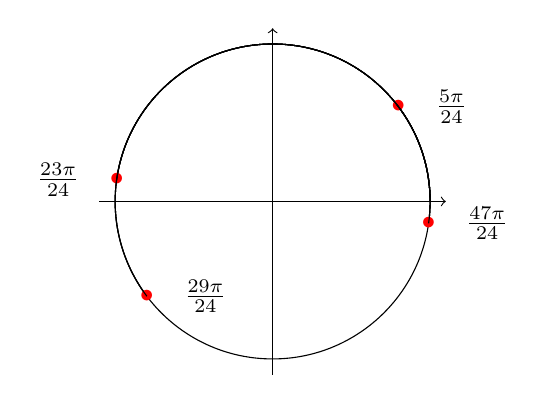
\begin{tikzpicture}[scale=2]
%Axes
\draw [->] (-1.1,0) -- (1.1,0);
\draw [->] (0,-1.1) -- (0,1.1);
%Cercle
\draw (0,0) circle (1);
%Points
\draw (1,0) arc (0:37:1) node [red] {$\bullet$};
\draw (1,0) arc (0:37:1) node[right] {$\quad \ddp \frac{5\pi}{24}$} ;
\draw (1,0) arc (0:-8:1) node [red] {$\bullet$};
\draw (1,0) arc (0:-8:1) node[right] {$\quad\ddp \frac{47\pi}{24} $} ;
\draw (1,0) arc (0:172:1) node [red] {$\bullet$};
\draw (1,0) arc (0:172:1) node[left] {$\ddp \frac{23\pi}{24}\quad $} ;
\draw (1,0) arc (0:217:1) node [red] {$\bullet$};
\draw (1,0) arc (0:217:1) node[right] {$\quad\ddp \ddp\frac{29\pi}{24}$} ;
\end{tikzpicture}
\end{center}
\end{minipage}
%--------------------------------------------------
\item \textbf{R\'esolution de $\mathbf{1+\cos{x}+\sin{(5x)}+\sin{(6x)}=0}$:}\\
\noindent On commence par transformer l'expression gr\^{a}ce au formulaire de trigonom\'etrie afin de la mettre sous forme factoris\'ee. On obtient
$$ 1+\cos{x}+\sin{(5x)}+\sin{(6x)}=2\cos^2{\left(  \ddp\frac{x}{2}\right)}+2\sin{\left(  \ddp\frac{11x}{2}\right)}\cos{\left(  \ddp\frac{x}{2}\right)}=2\cos{\left(  \ddp\frac{x}{2}\right)} \left(  \cos{\left(  \ddp\frac{x}{2}\right)}  +\sin{\left(  \ddp\frac{11x}{2}\right)} \right).$$
Ainsi r\'esoudre $1+\cos{x}+\sin{(5x)}+\sin{(6x)}=0$ est \'equivalent \`{a} r\'esoudre $\cos{\left(  \ddp\frac{x}{2}\right)}=0$ ou $\cos{\left(  \ddp\frac{x}{2}\right)}  +\sin{\left(  \ddp\frac{11x}{2}\right)} =0$. On peut d\'ej\`{a} r\'esoudre la premi\`{e}re \'equation et on obtient
$$ \cos{\left(  \ddp\frac{x}{2}\right)}=0 \Leftrightarrow\exists k\in\Z,\  \ddp\frac{x}{2}=\ddp\frac{\pi}{2}+k\pi\Leftrightarrow\exists k\in\Z,\  x=\pi+2k\pi.$$
\'Etudions la deuxi\`{e}me \'equation:
$$\hspace{-1cm} \begin{array}{lll}\cos{\left(  \ddp\frac{x}{2}\right)}  +\sin{\left(  \ddp\frac{11x}{2}\right)} =0 &\Leftrightarrow &\cos{\left(  \ddp\frac{x}{2}\right)} =-\sin{\left(  \ddp\frac{11x}{2}\right)} \Leftrightarrow \cos{\left(  \ddp\frac{x}{2}\right)} =\sin{\left( - \ddp\frac{11x}{2}\right)} \Leftrightarrow
\cos{\left(  \ddp\frac{x}{2}\right)} =\cos{\left(\ddp\frac{\pi}{2} + \ddp\frac{11x}{2}\right)}\vsec\\ &\Leftrightarrow&
\left\lbrace\begin{array}{lllll}
\exists k\in\Z, & \ddp\frac{x}{2}&=& \ddp\frac{\pi}{2} + \ddp\frac{11x}{2}+2k\pi\\
\hbox{ou}\\
\exists k\in\Z, & \ddp\frac{x}{2}&=& -\ddp\frac{\pi}{2} - \ddp\frac{11x}{2}+2k\pi
\end{array}\right. \Leftrightarrow \left\lbrace\begin{array}{lllll}
\exists k\in\Z, & x&=& -\ddp\frac{\pi}{10} - \ddp\frac{2k\pi}{5}\\
\hbox{ou}\\
\exists k\in\Z, & x&=& -\ddp\frac{\pi}{12} - \ddp\frac{k\pi}{3}.
\end{array}\right. \end{array}$$
Ainsi, on obtient 
\begin{equation*}
 \fbox{
 \begin{minipage}[t]{0.7\textwidth}
$\mathcal{S}=\left\lbrace  \pi+2k\pi,\ k\in\Z\right\rbrace\cup\left\lbrace   -\ddp\frac{\pi}{10} - \ddp\frac{2k\pi}{5}, \ k\in\Z\right\rbrace\cup\left\lbrace -\ddp\frac{\pi}{12} - \ddp\frac{k\pi}{3},\ k\in\Z\right\rbrace\\ \hbox{et}\  \mathcal{S}_{\lbrack 0,2\pi\lbrack}= \left\lbrace \ddp\frac{\pi}{4},\ddp\frac{3\pi}{10},\ddp\frac{7\pi}{12},\ddp\frac{7\pi}{10},\ddp\frac{11\pi}{12},\pi,\ddp\frac{11\pi}{10},\ddp\frac{15\pi}{12},\ddp\frac{15\pi}{10},\ddp\frac{19\pi}{12},\ddp\frac{19\pi}{10},\ddp\frac{23\pi}{12}            \right\rbrace.$
\end{minipage}}
\end{equation*}
%--------------------------------------------------
\item \textbf{R\'esolution de $\mathbf{\tan^4{x}+2\tan^2{x}-3=0}$:}\\
\noindent On pose le changement de variable $X=\tan^2{(x)}$ et on doit donc r\'esoudre: $X^2+2X-3=0$. Le calcul du discriminant donne que les solutions sont $-3$ et $1$. Ainsi, on doit r\'esoudre les deux \'equations $\tan^2{(x)}=-3$ et $\tan^2{(x)}=1$. Comme un carr\'e est toujours positif, la premi\`{e}re \'equation est impossible. La deuxi\`{e}me \'equation donne $\tan{(x)}=-1$ ou $\tan{(x)}=1$. \\
 \begin{minipage}[c]{0.45\textwidth}
On obtient donc
$$\fbox{$\mathcal{S}_{\R}=\left\lbrace -\ddp\frac{\pi}{4}+k\pi,\ k\in\Z \right\rbrace\cup\left\lbrace \ddp\frac{\pi}{4}+k\pi,\ k\in\Z \right\rbrace$}.$$
$$\fbox{$ \mathcal{S}_{\lbrack 0,2\pi\lbrack}= \left\lbrace \ddp\frac{\pi}{4},\ddp\frac{3\pi}{4},\ddp\frac{5\pi}{4},\ddp\frac{7\pi}{4}   \right\rbrace$}.$$
\end{minipage}
\quad \begin{minipage}[c]{0.45\textwidth}
\begin{center}
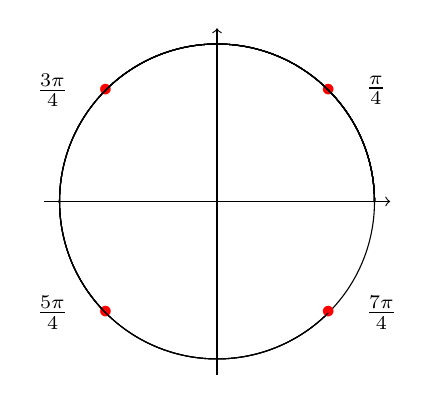
\begin{tikzpicture}[scale=2]
%Axes
\draw [->] (-1.1,0) -- (1.1,0);
\draw [->] (0,-1.1) -- (0,1.1);
%Cercle
\draw (0,0) circle (1);
%Points
\draw (1,0) arc (0:45:1) node [red] {$\bullet$};
\draw (1,0) arc (0:45:1) node[right] {$\quad\ddp \frac{\pi}{4}$} ;
\draw (1,0) arc (0:135:1) node [red] {$\bullet$};
\draw (1,0) arc (0:135:1) node[left] {$\ddp \ddp\frac{3\pi}{4}\quad$} ;
\draw (1,0) arc (0:225:1) node [red] {$\bullet$};
\draw (1,0) arc (0:225:1) node[left] {$\ddp \ddp\frac{5\pi}{4}\quad$} ;
\draw (1,0) arc (0:315:1) node [red] {$\bullet$};
\draw (1,0) arc (0:315:1) node[right] {$\quad \ddp \ddp\frac{7\pi}{4}$} ;
\end{tikzpicture}
\end{center}
\end{minipage}
\end{enumerate}
\end{correction}